\documentclass{article}
\usepackage[utf8]{inputenc}
\usepackage[margin = 0.8in]{geometry}
\usepackage{graphicx}
\usepackage{amsmath, amssymb}
\usepackage{subcaption}
\usepackage{multirow}
\usepackage{mathtools}
\usepackage{float}
\usepackage{pythonhighlight}


\title{RBE595 - Week 2 Programming Assignment}
\author{Keith Chester}
\date{Due date: January 22, 2023}

\begin{document}
\maketitle

This is a programming assignment where we were tasked with recreating a figure in our textbooks. The figure demonstrated the effects of modifying the $\epsilon$ for epsilon-greedy approaches. That figure and the code utilized to generate it is shared below:


\begin{figure}[H]
    \centering
    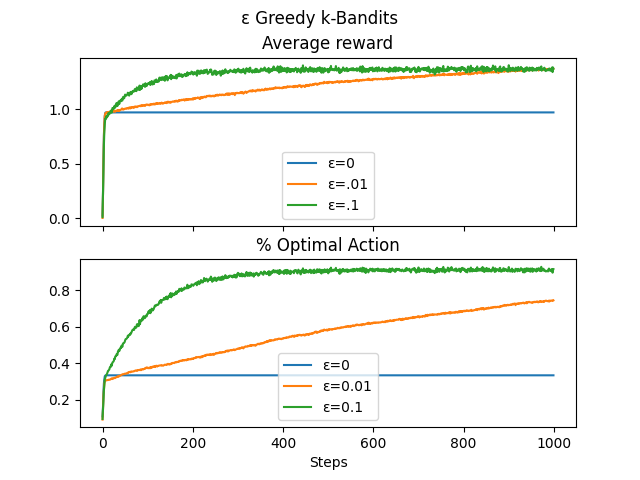
\includegraphics[width = 0.8\textwidth]{./epsilon_greedy.png}
    \caption{Recreated figure}
    \label{fig:chart}
\end{figure}



\begin{python}
from math import sqrt
from random import gauss, randint, uniform
from typing import List, Tuple

import matplotlib.pyplot as plt


def perform_run(
    steps: int, epsilon: float, k_bandits: int
) -> Tuple[List[float], List[int]]:
    """
    perform_run takes a given number of steps and an epsilon, and then takes
    that run for :steps: steps. Once this is done it returns a list of each
    rewards on that step, and whether or not it was the optimal action
    (represented as 0 or 1)
    """
    rewards: List[float] = []
    optimal: List[int] = []

    # We need to create a specified amount of bandits with mean 0
    # and variance 1 for our problem
    mean = 0
    variance = 1
    bandits = [gauss(mean, sqrt(variance)) for i in range(0, k_bandits)]
    best_bandit = bandits.index(max(bandits))
    # We assume some knowledge about the bandits. Over time we will learn
    # more as we explore.
    # knowledge = [gauss(mean, sqrt(variance)) for i in range(0, k_bandits)]
    knowledge = [1.0] * k_bandits

    for i in range(0, steps):
        if uniform(0, 1) <= 1 - epsilon:
            # In this situation we act greedily.
            index = knowledge.index(max(knowledge))
        else:
            # We explore here
            index = randint(0, k_bandits - 1)

        # Grab our reward
        reward = bandits[index]
        knowledge[index] = reward
        rewards.append(reward)
        # Is it optimal? Record that
        optimal.append(1 if index == best_bandit else 0)

    return rewards, optimal


def run_experiment(runs: int, steps_per_run: int, epsilon: float, k_bandits: int):
    all_rewards: List[float] = [0.0] * steps_per_run
    all_optimal: List[float] = [0.0] * steps_per_run

    for _ in range(0, runs):
        rewards, optimal = perform_run(steps_per_run, epsilon, k_bandits)

        # We are iterativeley calculating the all_rewards
        # and all_optimal averages so we can avoid holding
        # it all in memory
        for step, _ in enumerate(all_rewards):
            all_rewards[step] += rewards[step] / runs
            all_optimal[step] += optimal[step] / runs

    return all_rewards, all_optimal


if __name__ == "__main__":
    runs = 2000
    steps = 1000
    bandits = 10
    rewards_00, optimal_00 = run_experiment(runs, steps, 0.00, bandits)
    rewards_01, optimal_01 = run_experiment(runs, steps, 0.01, bandits)
    rewards_10, optimal_10 = run_experiment(runs, steps, 0.10, bandits)

    figure, axis = plt.subplots(2, sharex=True)
    plt.xlabel("Steps")
    figure.suptitle("E Greedy k-Bandits")

    axis[0].set_title("Average reward")
    axis[0].plot(rewards_00, label="E=0")
    axis[0].plot(rewards_01, label="E=.01")
    axis[0].plot(rewards_10, label="E=.1")
    axis[0].legend(loc="lower center")

    axis[1].set_title("% Optimal Action")
    axis[1].plot(optimal_00, label="E=0")
    axis[1].plot(optimal_01, label="E=0.01")
    axis[1].plot(optimal_10, label="E=0.1")
    axis[1].legend(loc="lower center")

    figure.savefig("./epsilon_greedy.png")


\end{python}


\end{document}